\newcommand{\mgamcnlo}{MG5\_aMC@NLO\xspace}
%~ \newcommand{\a}{a}
\newcommand{\A}{A}
%~ \newcommand{\maddm}{MADDM}

\subsection{\color{red} TODO}
\begin{itemize}
\color{red}

\item{\textbf{General}}
    \subitem{Polish text.}
    \subitem{Need very clear statements about what parameters are used. This will probably already be described elsewhere.}
\item{\textbf{2D \mDM-\mA scan}}
    \subitem{Done.}
\item{\textbf{1D \mDM scan}}
    \subitem{Beautify plot.}
    \subitem{Add description in text}
\item{\textbf{Add other scans?}}

\end{itemize}

\subsection{Actual content}

An important requirement for models of dark matter is their consistency with existing astrophysical observations, namely the observed dark matter relic density.
The relic density is driven by the annihilation cross-section of dark matter into SM particles.
For a given model of dark matter-SM interactions, the annihilation cross-section is fully defined and a calculation of the resulting relic density can be performed. 

We use the \maddm~\cite{Backovic:2013dpa,Backovic:2015cra} plugin for \mgamcnlo in oder to calculate the present-day relic density for this model. By modeling the thermal evolution of the cross-section during the expansion of the early universe, the time of freeze-out is determined. All tree-level annihilation processes are taken into account , and the Yukawa couplings of all fermions are taken to be non-zero. The Feynman diagrams of annihilation processes taken into account in this calculation are shown in fig.~\ref{fig:feyn_annihilation}. Generally, the annihilation proceeds via single or double s-channel exchange of the pseudoscalars a and A, with subsequent decays. Since \maddm uses only tree-level diagrams, contributions from off-shell pseudoscalars can only be taken into account for the case of single s-channel mediation with direct decay of the pseudoscalar to SM fermions. If the pseudoscalar instead decays to other bosons or if the annihilation proceeds through double s-channel diagrams, the outgoing bosons are taken to be on-shell and their decays are not simulated. 

The relic density is shown for a scan in the \ma-\mDM plane in fig.~\ref{fig:relic_scan_mxd_ma}.
For small values of $\mDM$ below the mass of the top quark, DM is mostly overabundant. In this regime, annihilation to quarks is suppressed by the small Yukawa couplings of the light fermions. The observed relic density can only be achieved for $\mDM\approx\ma/2$, where annihilation is resonantly enhanced, or for $\mDM \approx (\ma+\mh)/2$, close to the threshold for the $\chi\chi\rightarrow h a$ process.
Above the top threshold, annihilation into fermions becomes very efficient and DM is underabundant. As \mDM increases further, annihilation via single s-channel diagrams is increasingly suppressed and the relic density rises again. The observed density is reproduced again for $\mDM\approx1 \mathrm{TeV}$ at low \ma.

\begin{figure}[h]
\centering
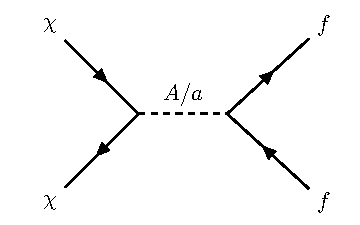
\includegraphics[]{texinputs/05_relic/figures/feynman/graph_2hdm_relic_s_fermions.pdf}
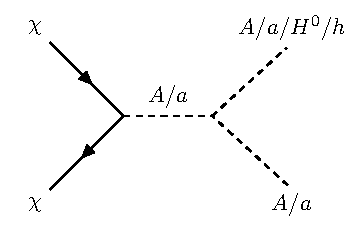
\includegraphics[]{texinputs/05_relic/figures/feynman/graph_2hdm_relic_s_bosons.pdf}
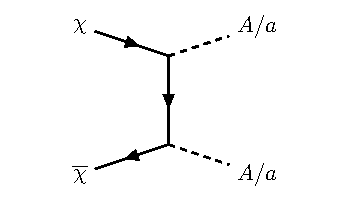
\includegraphics[]{texinputs/05_relic/figures/feynman/graph_2hdm_relic_ss_bosons.pdf}
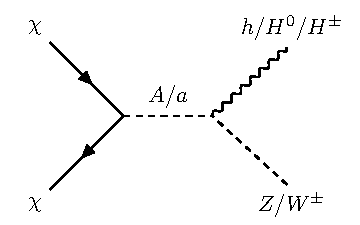
\includegraphics[]{texinputs/05_relic/figures/feynman/graph_2hdm_relic_s_vbosons.pdf}
\label{fig:feyn_annihilation}
\caption{Annihilation diagrams taken into account in the relic density calculation.}
\end{figure}

\begin{figure}[h]
\centering
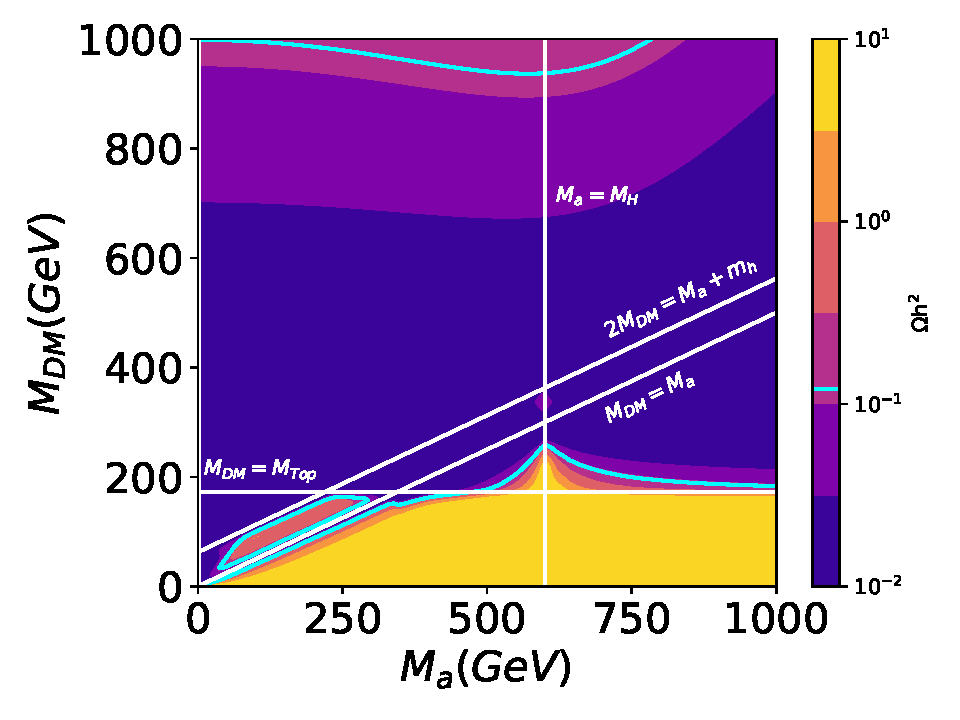
\includegraphics[width=0.8\textwidth]{{texinputs/05_relic/figures/relic/contour_scan_mxd_ma.pdf}}
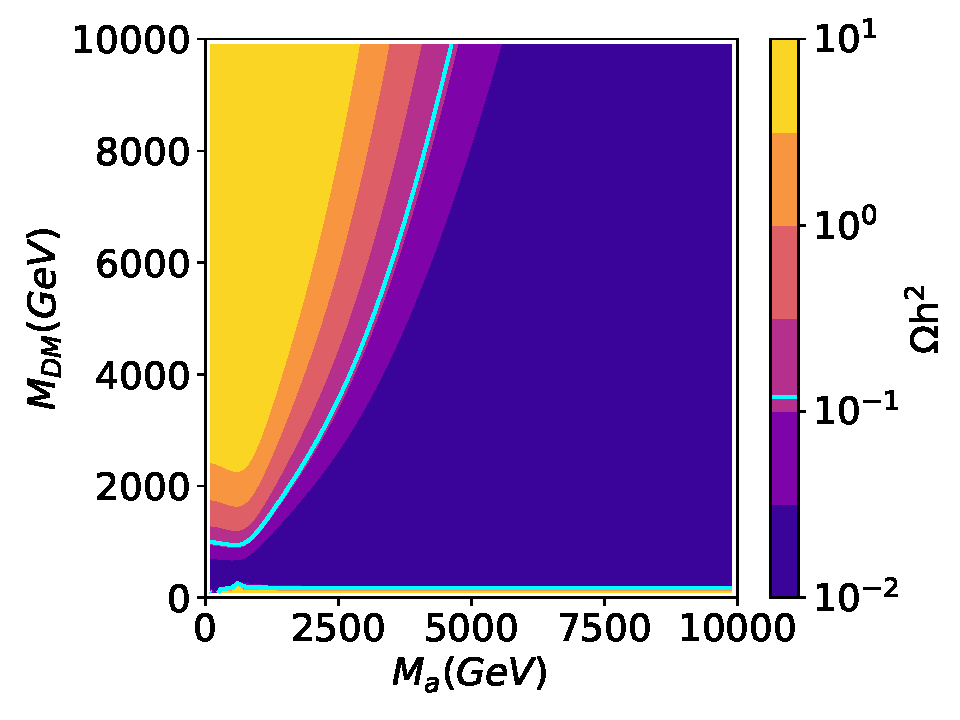
\includegraphics[width=0.8\textwidth]{{texinputs/05_relic/figures/relic/contour_scan_mxd_ma_large.pdf}}
\label{fig:relic_scan_mxd_ma}

\caption{Predicted relic density for a two-dimensional scan of \mDM and \ma. The color scale indicates the relic density, the cyan solid line shows the observed value of $\Omega h^{2} = 0.12$. The color scale is truncated at its ends, i.e. values larger than the maximum or smaller than the minimum are shown in the same color as the minimum / maximum. While the top panel focuses on the mass region relevant to collider searches, the bottom panel shows the development of the relic density for a larger mass region.}
\end{figure}

\begin{figure}[h]
\centering
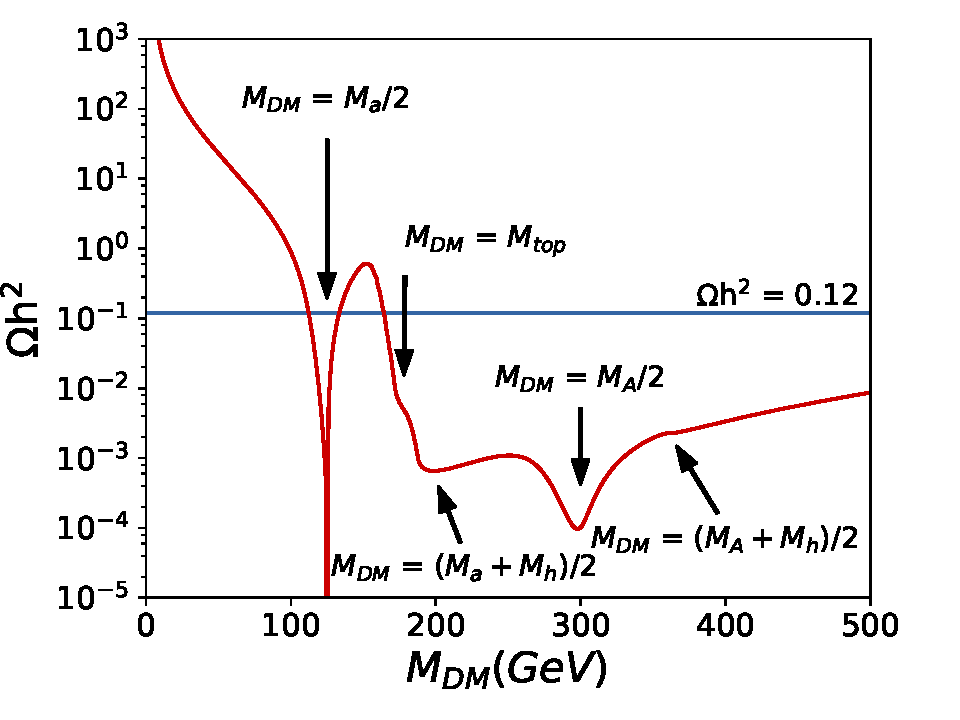
\includegraphics[]{texinputs/05_relic/figures/relic/line_scan_mdm.pdf}
\caption{Relic density for a one-dimensional scan of \mDM.}
\end{figure}
